% ---------------------------------------------------------------------
% Manuscript for the Journal of Computational Biology (SAGE Publishing;
% formerly Mary Ann Liebert, Inc.). Research Article. Initial submission as
% a full-text PDF; double-spaced, 12 pt Times, single column. In-text
% citations use author-year and the reference list follows the Sage Harvard
% style (unnumbered). This file is fully anonymised for double-anonymized
% review; identifying information is on the separate title page.
% ---------------------------------------------------------------------
\documentclass[12pt]{article}
\usepackage[T1]{fontenc}
\usepackage{times}      % Times text font (standard math)
\renewcommand{\ttdefault}{cmtt}   % Courier metrics unavailable on this TeX install
\usepackage{setspace}
\usepackage[margin=1in]{geometry}
\usepackage{amsmath,amssymb}
\usepackage{graphicx}
\usepackage{booktabs}
\usepackage{array}
\usepackage[hidelinks]{hyperref}

\doublespacing
\setlength{\parindent}{1.5em}
\setlength{\parskip}{0pt}

\begin{document}

\begin{center}
{\LARGE\bfseries The Breast Cancer Gene Network as a Complex
Adaptive System: Controllability, Feedback Structure and Relapse-Free
Survival in METABRIC, with Cross-Cohort Transportability Assessment in
TCGA-BRCA}
\end{center}

\vspace{0.4em}
\begin{center}
\textit{[Anonymised for double-anonymized review; author and affiliation
are provided on the title page]}\\
\end{center}

\vspace{0.4em}
\begin{center}
\textbf{Running title:} Cybernetic control-kernel score and breast cancer
prognosis\\
\textbf{Keywords:} breast cancer; gene association network; controllability;
control energy; survival analysis; graphical lasso
\end{center}

\vspace{0.6em}

\begin{center}
\textbf{Abstract}
\end{center}

\textbf{Background:} Cancer progression is often described as the behaviour of
a complex adaptive system; we ask whether control-theoretic descriptors of
its transcriptional association network carry incremental prognostic
information beyond conventional clinical variables. \textbf{Methods:} From
1,979 METABRIC primary tumours we inferred a sparse 99-gene
conditional-dependence network, computed cybernetic descriptors and built a
patient-level control-kernel score (CS) with structure-based, outcome-blind
weights. CS was tested against relapse-free survival (RFS) by Cox, repeated
and full-pipeline cross-validation, log-rank, permutation, Bayesian
horseshoe and Schoenfeld proportional-hazards analyses; cross-cohort
transportability was assessed in TCGA-BRCA (n = 710) on overall survival
(OS). \textbf{Results:} The inferred network is cycle-rich (242 independent
undirected cycles), stable under dissipative realisation (spectral radius
0.904, damping $\eta$ = 1.2), and requires 24 independent driver channels
(75-dimensional controllable subspace). CS was associated with RFS after
adjustment (HR 1.22 per SD, p = $5.6\times10^{-6}$), with strongly
time-dependent effect (Schoenfeld p = $2.0\times10^{-14}$): HR per SD 1.65 within
0--24 months, 1.29 within 24--60, 0.91 after 60. Full-pipeline
cross-validation improved the C-index from 0.587 $\pm$ 0.041 (clinical) to
0.606 $\pm$ 0.031 (+CS); on the fixed network, 0.588 to 0.611. In
TCGA-BRCA, CS showed no association with OS (HR 1.00, 95\% CI 0.80--1.25,
p = 0.99), and the inferred network did not reproduce across cohorts
(Jaccard index 0.02--0.04). \textbf{Conclusions:} A score derived from the network's
structural control kernel carries prognostic information for RFS in
METABRIC, but the association is cohort- and endpoint-specific and
time-dependent; an observational conditional-dependence network should not
be interpreted as a causal, portable regulatory programme.

\section{Introduction}

Since Wiener's formulation of cybernetics as the science of control and
communication in animals and machines (Wiener 1948), the language of
feedback, stability and control has proved remarkably productive in biology
(Thomas et al.\ 2019). Gene regulatory networks (GRNs) are prototypical
cybernetic objects: their function emerges from dense feedback wiring, their
operating point is maintained by homeostatic (negative-feedback) circuits,
and their collective behaviour can be analysed with the tools of linear and
nonlinear control theory (Liu and Barab\'asi 2016; Za\~nudo et al.\ 2017).
At the same time, cancer is increasingly framed as a complex adaptive
system---a multilevel, self-organising network whose phenotypic states
correspond to stable attractors of the underlying molecular dynamics (Li and
Bal\'azsi 2018; Feinberg and Levchenko 2023; Shin and Cho 2023; Berner et
al.\ 2023). In this view a tumour is not a fixed molecular entity but a
dynamical regime of a regulatory network, and recurrence or resistance can
be interpreted as transitions between attractors.

Breast cancer is a natural test bed for this systems-level perspective.
Large transcriptomic cohorts such as METABRIC (Curtis et al.\ 2012) have
made it possible to reconstruct condition-specific gene networks from
patient-level expression data and to link network structure to clinical
outcome (Nersisyan et al.\ 2021; Wang and Liu 2022; Huo et al.\ 2022). A
recurring finding is that the topology of the inferred network---rather than
any single gene---carries prognostic signal: rewiring analyses (Wang and Liu
2022) and network-driven survival analyses of breast cancer transcriptomes
(Nersisyan et al.\ 2021; Huo et al.\ 2022) associate network-level features
with outcome, while Boolean-model studies characterise the attractor
structure of the inferred regulatory programme (Sgariglia et al.\ 2021). Established multigene expression signatures already translate
gene-expression measurements into prognosis (Hatzis et al.\ 2011), but what
is missing is a direct link from the control-theoretic descriptors of network
structure---controllability,
control energy and structural cycle richness (Liu et al.\ 2011; Yuan et
al.\ 2013; Gao et al.\ 2014; Yan et al.\ 2015)---to patient-level survival
models. This
study provides such a link by translating a purely structural control
analysis of the breast cancer GRN into a patient-level prognostic score.
Throughout, we use the term \emph{GRN} as a computational shorthand for the
inferred gene-level conditional-dependence network, not as a claim of a
causal, experimentally verified regulatory map.

An important epistemic distinction frames the analysis and its
interpretation. (i) The network is an \emph{observational conditional-
dependence structure} estimated from cross-sectional expression; it does
not claim to be a causal, experimentally verified regulatory programme.
(ii) The network descriptors are \emph{structural properties} of that
estimated object---cycle-space dimension, spectral stability,
controllability and control-energy budgets---computed without any access to
clinical outcome.
(iii) The patient score is a \emph{control-energy-inspired summary} of
expression projected onto the network's control kernel. (iv) Any
association of the score with survival is an \emph{empirical prognostic
association} whose generalisability must be demonstrated, not assumed.
We keep these four levels separate throughout: in particular, we do not
claim that the inferred network is the physical control system of the cell,
nor that the score is a causal determinant of outcome. Cross-cohort assessment
in an independent cohort is treated as a decisive test of the fourth level.

In this paper we address three questions. (i) What is the cybernetic
organisation of the breast cancer GRN inferred from a large expression
cohort? (ii) Viewed as a complex adaptive system, is the inferred network
dynamically stable, and does its dynamical regime support a multistable-
attractor view of tumour phenotypes or a single, homeostatic operating
point? (iii) Does a patient-level score derived from the control-kernel
structure, computed without access to clinical outcome, carry prognostic
information for relapse-free survival (RFS) after adjustment for standard
clinical covariates---and does that association transport to an independent
cohort?

\section{Materials and Methods}

\subsection{Data and Pre-processing (METABRIC)}

We analysed mRNA expression and clinical data from the Molecular Taxonomy of
Breast Cancer International Consortium (METABRIC) cohort (Curtis et al.\
2012; Rueda et al.\ 2019), a collection of primary invasive breast tumours
with long-term follow-up. Expression values were downloaded from the
cBioPortal data repository (study \texttt{brca\_metabric}). Following
quality control, 1,979 tumours with complete expression data for 99
a-priori breast-cancer regulatory genes were retained. The gene set spans
the principal regulatory axes of breast cancer biology: oestrogen receptor
signalling (ESR1, PGR), epidermal growth factor receptor signalling (EGFR,
ERBB2/HER2), PI3K/AKT/mTOR signalling, cell-cycle control (CDK1, CCNA2, CCNB1, CCNB2,
CCND1/2, CCNE1, MYC), the p53/DNA-damage response (TP53, MDM2), apoptosis
and EMT regulators, and core transcription factors (Supplementary Table
S1).
Per-gene expression was z-score standardised across samples. Clinical
covariates comprised oestrogen receptor (ER), progesterone receptor (PR)
and HER2 status, histological grade and age at diagnosis (PR status missing
for two patients and HER2 status for one; Table~1). The primary endpoint
was relapse-free survival (RFS), defined as the time to any invasive relapse
event or last follow-up.

\subsection{Conditional-Dependence Network Inference}

We inferred a sparse, undirected conditional dependence network among the 99
genes with the graphical lasso (Friedman et al.\ 2008), which estimates the
precision (inverse covariance) matrix $\boldsymbol{\Theta}$ by
\begin{equation}
\hat{\boldsymbol{\Theta}} = \arg\max_{\boldsymbol{\Theta}\succ 0}
\left\{ \log\det\boldsymbol{\Theta} - \operatorname{tr}
(\mathbf{S}\boldsymbol{\Theta}) - \alpha\|\boldsymbol{\Theta}\|_1 \right\},
\end{equation}
where $\mathbf{S}$ is the sample covariance of the z-scored expression
matrix and the penalty $\alpha$ was selected by 3-fold cross-validation
over six candidate values. Partial correlations were derived as
$\pi_{ij} = -\hat{\Theta}_{ij}/\sqrt{\hat{\Theta}_{ii}\hat{\Theta}_{jj}}$;
an edge $(i,j)$ was declared present when $|\pi_{ij}| > 0.05$ for the sparse
network, and the full weighted graph used the absolute partial correlations
above $10^{-12}$ for the topological and control analyses. Edge stability
was assessed by re-estimating the network on 25 bootstrap resamples (80\% of
samples each) and recording the fraction of resamples in which each inferred
edge reappeared.

\subsection{Cybernetic Network Metrics}

Let $G=(V,E)$ be the inferred GRN with $N=|V|$ genes, $E=|E|$ edges and $C$
connected components. Three cybernetic descriptors were computed.
(i) \emph{Cycle-space dimension:} the cyclomatic number $M = E - N + C$
counts the independent undirected cycles of the graph. In an undirected
conditional-dependence network these cycles do not by themselves identify
directed regulatory feedback loops; they measure the structural capacity of
the graph to support closed-loop control were directionality known.
(ii) \emph{Spectral stability:} for the weighted adjacency matrix
$\mathbf{A}$ with entries $|\pi_{ij}|$, the local stability of the
linearised dissipative dynamics $\dot{\mathbf{x}} = (\mathbf{A} -
\eta\mathbf{I})\mathbf{x}$ is governed by the spectrum of $\mathbf{A}$;
choosing dissipation $\eta > \rho(\mathbf{A})$ places the spectrum in the
left half-plane. (iii) \emph{Controllability:} for the linear dynamics
$\dot{\mathbf{x}} = \mathbf{A}\mathbf{x} + \mathbf{B}\mathbf{u}$, the
minimum number of independent input channels equals the largest geometric
multiplicity of any eigenvalue of $\mathbf{A}$ (Yuan et al.\ 2013); for the
symmetric matrix inferred here this maximum multiplicity is the
$N - \operatorname{rank}(\mathbf{A}) = 24$-dimensional zero eigenspace. As a structure-based proxy for the nodes most relevant
to steering the network state, we ranked genes by a combined control score
$c_i$ equal to the mean of the percentile ranks of degree, betweenness
centrality and eigenvector centrality; the \emph{control kernel} was defined
as the top 60 ranked genes. This kernel is a centrality-based structural
proxy and is distinct from the minimum driver set of the exact-controllability
analysis; the two notions are kept separate throughout.

\subsection{Control Energy}

We modelled the linearised, dissipative network dynamics
\begin{equation}
\dot{\mathbf{x}}(t) = (\mathbf{A} - \eta \mathbf{I})\,\mathbf{x}(t)
+ \mathbf{B}\,\mathbf{u}(t),
\end{equation}
with dissipation $\eta = 1.2 > \rho(\mathbf{A})$ and input matrix
$\mathbf{B}$ selecting the control-kernel genes. The controllability Gramian
$\mathbf{W}_c$ solves the continuous Lyapunov equation
$\mathbf{A}_\eta \mathbf{W}_c + \mathbf{W}_c\mathbf{A}_\eta^\top =
-\mathbf{B}\mathbf{B}^\top$, with $\mathbf{A}_\eta = \mathbf{A} - \eta
\mathbf{I}$. Because the kernel inputs drive only 75 of the 99 state
dimensions, $\mathbf{W}_c$ is singular; we report its spectrum in the
reachable subspace, truncate eigenvalues below $10^{-12}$ for display, and
state the dimension of the controllable subspace explicitly. The minimum
energy required to steer the system from the origin to a target state
$\mathbf{x}_f$ in the controllable subspace is $E_{\min} =
\mathbf{x}_f^\top \mathbf{W}_c^{+}\mathbf{x}_f$, where the pseudo-inverse
$\mathbf{W}_c^{+}$ is evaluated numerically as the inverse of the
regularised Gramian $\mathbf{W}_c + \delta\mathbf{I}$, with $\delta =
10^{-6}\,\operatorname{tr}(\mathbf{W}_c)/N$ (here $\delta =
2.7\times10^{-7}$); the pseudo-inverse is recovered in the limit
$\delta\to 0$. We report the eigenvalue spectrum of $\mathbf{W}_c$, its
condition number, its effective rank (number of eigenvalues above $10^{-6}$
of the maximum) and the fraction of the total Gramian trace carried by the
top 10\% of modes, which quantifies how concentrated the inexpensive control
channels are (Yan et al.\ 2015). For each kernel gene we also computed the
trace of the single-input Gramian as a per-driver measure of
controllability.

\subsection{Dynamical Simulation and Convergence Analysis}

The inferred network was treated as a complex adaptive system in two
complementary simulation regimes. (i) \emph{Linear dissipative regime:} we
integrated Eq.~(2) from 40 random initial states and projected the terminal
states onto the Perron eigenvector of $\mathbf{A}$ (normalised to unit
sum), obtaining a scalar phenotype coordinate; the projections at the
horizon were split at the sample median into low- and high-response halves
that define two response poles used for the constant-input perturbation
experiment. (ii) \emph{Nonlinear saturating regime:} we integrated
$\dot{\mathbf{x}} = -\mathbf{x} + \tanh(\mathbf{A}\mathbf{x}) +
\mathbf{B}\mathbf{u}$ from random initial states (drawn independently for
the two regimes) and partitioned the
terminal projections into three bands by tertiles to characterise transient
spread. To test whether these bands correspond to distinct attractors, we
located fixed points of the nonlinear system by fixed-point iteration and
multi-start root finding and assessed their local stability from the
Jacobian spectrum. In addition, we ran a constant-input perturbation
experiment: starting from the state with the lowest transient projection,
we applied the constant input $\mathbf{u}_{\mathrm{const}} =
\mathbf{B}^{\top}\mathbf{W}_c^{+}\Delta$ (regularised Gramian; $\Delta$
the difference between the lowest and highest projection states), integrated
the linearised dynamics over a horizon of $T = 8$, and compared the
resulting trajectory with the uncontrolled trajectory from the same initial
state. We report the integrated input energy $\int_0^T \|\mathbf{u}\|^2
\mathrm{d}t$, the endpoint projection, the full-state error relative to the
target, and whether the uncontrolled run also crosses the median projection
line. This experiment is presented as a demonstration of input-modulated
transient response only; it is not claimed to be a minimum-energy steering
or a phenotype-transfer result.

\subsection{Control-Kernel Patient Score}

For each patient $s$ we defined the control-kernel score
\begin{equation}
\mathrm{CS}_s = \frac{\sum_{k \in \mathcal{K}} c_k\, z_{sk}}
{\sum_{k \in \mathcal{K}} c_k},
\end{equation}
where $\mathcal{K}$ is the control kernel, $z_{sk}$ is the z-scored
expression of gene $k$ in patient $s$, and $c_k$ is the structure-based,
outcome-blind control score of gene $k$. Crucially, $c_k$ is computed from
the network topology only, so $\mathrm{CS}_s$ contains no information about
survival or recurrence. The control-energy analysis of Section~2.4 motivates
the kernel as a set of structurally influential genes; the score itself uses
only the centrality weights and no dynamic or energy quantities, so that the
prognostic analysis tests the structural hypothesis rather than a fitted
dynamical model. The kernel size
$K = 60$ was pre-specified as the top $K$ genes by the control score before
any model fitting; the sensitivity of the association to $K$ is reported in
Section~3.6. The score was standardised across patients (mean 0, unit SD)
for interpretation.

\subsection{Survival Models and Inference (METABRIC)}

All models were estimated on the 1,979 patients with complete RFS and
expression data. The Cox proportional-hazards model (Cox 1972) was fitted
by maximising the partial likelihood (Breslow tie handling) with an analytic
gradient and BFGS optimisation; standard errors were obtained from the
BFGS quasi-Newton approximation to the inverse Hessian of the negative
partial log-likelihood, and the Harrell concordance index (C-index) was used
for discrimination. Grade and age were z-scored across the analysis sample,
and the 88 missing grade values were imputed to the z-score mean (zero). As
an independent check, the Cox coefficients, standard errors and confidence
intervals were re-estimated with the R \emph{survival} package (R 4.5.2,
survival 3.8.3, Efron tie handling), which computes the observed
information matrix exactly, and agreed with the Python estimates at the
reported precision. Three nested specifications were compared: M0 (clinical
covariates only: ER, PR, HER2, grade, age), M1 (M0 + CS) and M2 (Ridge-Cox
on the top 40 kernel-gene expressions plus clinical covariates, ridge
penalty 0.08). Discrimination was evaluated with repeated 5-fold
cross-validation (5 repeats, 25 splits in total, stratified by the event
indicator), reporting mean and SD of the C-index. Because the network, the
kernel genes, the CS weights and the clinical encoding are constructed once
on the full cohort in the main analysis, we additionally ran a full-pipeline
5-fold cross-validation in which every feature-construction step (expression
standardisation, graphical-lasso inference, centrality computation, kernel
selection, CS computation and clinical encoding) was refitted inside each
training fold and applied to the held-out fold; this second protocol
measures generalisation of the complete pipeline to unseen patients.
Survival differences between CS-high and CS-low strata (median split) were
tested with the log-rank test (Mantel--Cox form, with the standard variance
estimator) and displayed as Kaplan--Meier curves. The survival association
of CS was additionally tested with a permutation test in which the CS vector
was permuted 1,000 times while the survival times and event indicators were
held fixed, the univariate Cox model for CS was refitted on each permuted
score, and the observed CS coefficient was compared with its permutation
distribution; the reported p-value uses the finite-resolution correction
$(r+1)/(B+1)$. Finally, as a secondary exploratory analysis, we fitted a
Bayesian logistic model of 5-year relapse with a horseshoe prior on the
kernel-gene coefficients (Polya--Gamma Gibbs sampler, 4,000 iterations, 1,000
burn-in, sparsity scale p0 = 5; sensitivity p0 = 2 and 10 reported in
Results) and report posterior means, standard deviations and the area under
the ROC curve (AUC). The 5-year binary endpoint is defined only for patients
evaluable at 60 months (follow-up $\geq$ 60 months, or relapse before 60
months); the 144 patients censored before 60 months without relapse have
unknown 5-year outcome and are excluded, so the fixed-time model is a
complete-case analysis with an informative-censoring caveat and is
interpreted as exploratory only. Finally,
to separate the contribution of the network-based gene selection from the
prognostic content of any 60-gene set, we compared CS with (i) an
equal-weight average of the same 60 kernel genes and (ii) two null
distributions of 2,000 random 60-gene sets each (fixed seed), both drawn
from the same 99-gene panel from which the kernel was selected: random
genes with equal weights, and random genes with random rank-based weights.
The two nulls separate the effect of the gene-selection scheme (network
topology versus random choice within the same candidate panel) from the
effect of the weighting scheme (centrality ranks versus random ranks). A
whole-transcriptome null used in an earlier draft was dropped because it
draws from a different candidate universe and is not an apples-to-apples
comparison. To
characterise the time structure of the association, we checked the
proportional-hazards assumption with Schoenfeld residuals (R
\emph{survival}::cox.zph) on the M1 model, fitted a CS $\times$ log(1 $+$
time) interaction model, and estimated period-specific CS hazard ratios in
time splits at 24 and 60 months (survSplit; the few events recorded at 0
months were shifted to 0.01 month so that the left boundary lies strictly
below all observed times). Time-dependent discrimination was summarised by
Uno's inverse-probability-of-censoring AUC at 1, 3, 5 and 10 years, with
the censoring distribution estimated by Kaplan--Meier. Finally, we
quantified the overlap of CS with established clinical covariates by Pearson
correlation with ER, PR, HER2, grade and age.

\subsection{Cross-Cohort Transportability Assessment in TCGA-BRCA}

To assess whether the prognostic association of CS transports across
cohorts, we analysed The Cancer Genome Atlas breast carcinoma
cohort (TCGA-BRCA; The Cancer Genome Atlas Network 2012). Level-3 RNA
sequencing expression (HiSeqV2, RSEM-normalised) and the clinical matrix
were downloaded from the UCSC Xena platform (Goldman et al.\ 2020). Tumour
samples (sample type code 1) were retained. Of the 99 genes in the
METABRIC panel, 98 were present in the TCGA expression matrix (CXCL8 absent;
the 60-gene kernel retained 59 of 60 genes). Per-gene expression was
z-scored within TCGA, and CS was computed with the \emph{fixed} METABRIC
kernel weights $c_k$ (Eq.~3), so the score construction used no TCGA
survival information. TCGA-BRCA has no curated relapse-free-survival
endpoint; we therefore assessed transportability against overall survival (OS) in days,
constructed from vital status and follow-up days. The validation models
replicated the METABRIC specifications: a clinical baseline (ER, PR, HER2
by immunohistochemistry, age; there is no grade variable in the TCGA
clinical matrix) and a clinical + CS model. All survival statistics were
computed with the R \emph{survival} package (Cox partial likelihood, Efron
tie handling; concordance; log-rank test on the median split; 5-year
Kaplan--Meier estimates). This is therefore a cross-cohort
transportability assessment on a different endpoint (OS rather than RFS) and a different
platform (RNA-seq rather than microarray); we report it as such and discuss
the endpoint and platform differences explicitly.

\subsection{Cross-Cohort Network Structure Replication}

Because the CS weights are derived from the METABRIC network structure, the
portability of the score depends in part on whether the inferred network
structure itself is reproducible in an independent cohort. We re-estimated
the graphical-lasso network on the TCGA tumour samples (same 98-gene panel,
same regularisation protocol: 3-fold cross-validation, six candidate
penalties, $|\pi_{ij}| > 10^{-12}$ for the weighted graph and $|\pi_{ij}|
> 0.05$ for the sparse graph) and compared the two edge sets by the Jaccard
index on the shared gene set. This analysis is reported as a structural
replication check, not as evidence about causal regulation.

All analyses were performed with Python 3.14 (numpy, scipy, scikit-learn,
networkx, matplotlib) and R 4.5.2 (survival 3.8.3). The complete
pipeline---data download, network inference, control-theoretic metrics,
simulations, survival models and cross-cohort assessment---is available in the
accompanying code repository and reproduces every figure and table in this
paper.

\section{Results}

\subsection{Cohort and Clinical Profile (METABRIC)}

After quality control, 1,979 METABRIC tumours with complete RFS and
expression data formed the analysis set. During follow-up, 803 relapse
events were recorded (event rate 40.6\%; median follow-up exceeding 10 years
for censored patients). Consistent with established clinical knowledge, ER
status, HER2 status and grade stratified outcome in the expected directions:
the 5-year relapse rate was 22.6\% among ER-positive tumours versus 40.6\%
among ER-negative tumours, and 43.9\% among HER2-positive versus 24.6\%
among HER2-negative tumours; the corresponding Kaplan--Meier estimates of
the 5-year relapse probability ($1 - \hat{S}(60)$) were 21.6\%, 39.2\%,
42.1\% and 23.5\%, respectively; ER-positive patients had a markedly longer
median observed RFS (105.9 months) than ER-negative patients (79.0 months).
These 5-year relapse rates use a KM-style denominator (patients evaluable at
60 months) and are distinct from the follow-up-wide RFS event rates reported
in Table~1 (39.5\% versus 22.6\% for ER-positive, 43.9\% versus 40.6\% for
ER-negative, 52.2\% versus 43.9\% for HER2-positive, and 38.9\% versus
24.6\% for HER2-negative). Table~1 summarises the clinical profile of the
analysis set, and Fig.~1 shows the cohort composition by RFS event, ER
status and PR status.

\subsection{The Inferred GRN and its Cybernetic Organisation}

Graphical-lasso inference with cross-validated regularisation ($\alpha =
0.345$) yielded a sparse conditional dependence network among the 99
regulatory genes: 317 undirected edges out of 4,851 possible pairs (density
0.065), organised into 24 connected components and 27 greedy-modularity
communities, with a mean degree of 6.40 and a mean clustering coefficient of
0.37. The largest connected component contains 76 genes and all 317 edges;
the remaining 23 genes (including TP53, MDM2, CDKN1A, BAX, BAD, CASP9,
KRAS, BRAF, VEGFA and VEGFB) are isolated in the weighted graph. Edge
stability over 25 bootstrap resamples depends on the edge-reappearance
criterion. If an edge is considered present whenever its partial-correlation
magnitude exceeds $10^{-12}$ (the threshold of the weighted graph), mean
stability is high (0.947 across the 317 inferred edges) and 283 of 317
edges (89\%) reappeared in more than 80\% of resamples; the most stable
edges were centred on the oestrogen receptor (ESR1--PGR, ESR1--AR,
ESR1--TFF1, ESR1--ERBB3, ESR1--EGFR and ESR1--IGF1R, each with stability
1.00), and the ESR1--PGR edge is a textbook ER-signalling module. If edges
are instead required to clear the sparsity threshold $|\pi_{ij}| > 0.05$
used for the sparse graph, stability is much lower (mean 0.442, median 0.16;
only 120 of 317 edges reappeared in more than 80\% of resamples), and all
25 bootstrap fits emitted scikit-learn ``ConvergenceWarning'' notices from
the graphical-lasso estimator; we therefore treat
only the aggregate topological statistics as stable and caution against
over-reading any individual edge. Fig.~2 shows this largest component with
the control-kernel genes highlighted.

As a cybernetic system, the inferred network exhibits substantial cyclic
structure: its cyclomatic number $M = E - N + C = 317 - 99 + 24 = 242$
implies 242 independent undirected cycles, i.e.\ a cycle-space dimension of
2.44 per gene. In an undirected conditional-dependence graph these cycles do
not identify directed regulatory feedback loops; they indicate the
structural capacity of the network to support feedback wiring and
closed-loop homeostasis (Wiener 1948). The linearised dynamics
$\dot{\mathbf{x}} = \mathbf{A}\mathbf{x}$ on the weighted network have
spectral radius $\rho(\mathbf{A}) = 0.904$ (largest eigenvalue 0.904,
smallest $-0.422$; Fig.~3, right); with dissipation $\eta = 1.2 >
\rho(\mathbf{A})$, all eigenvalues of the stabilised matrix
$\mathbf{A} - \eta\mathbf{I}$ lie in the left half-plane
($\operatorname{Re}\lambda \leq -0.296$), so the unforced linearised system
is asymptotically stable: perturbations to the regulatory state decay, the
dynamical signature of a homeostatic network operating near a stable
operating point. For the controllability analysis, the weighted adjacency
matrix has rank 75, so by the exact-controllability result for symmetric
matrices (Yuan et al.\ 2013) the minimum number of independent input
channels is $N - \operatorname{rank}(\mathbf{A}) = 24$, corresponding to
the 24-fold zero eigenspace; this is far smaller than the naive count
$N - \mu(\lambda_{\max}) = 98$ that would apply if the largest-eigenvalue
multiplicity were the binding constraint, and it confirms that only the zero
eigenspace (the 23 isolated genes and one extra redundant mode) is
unreachable in principle. We used the top 60 genes by structural centrality
(the control kernel) rather than the minimum input set to define the
patient-level score, because the centrality ranking is continuous and
reflects the relative importance of genes in steering the network; with
these 60 inputs the reachable subspace has dimension 75 of 99, i.e.\ the 23
isolated, undriven genes are not controllable from the kernel inputs.

\subsection{Control Energy of the Stabilised Network}

For the dissipative dynamics $\dot{\mathbf{x}} = (\mathbf{A} -
1.2\,\mathbf{I})\mathbf{x} + \mathbf{B}\mathbf{u}$, the controllability
Gramian over the 60-gene control kernel has rank 75, i.e.\ the kernel inputs
render a 75-dimensional subspace of the 99-dimensional state space
controllable. Within the reachable subspace the smallest nonzero Gramian
eigenvalue is $3.06\times10^{-8}$ and the dynamic range
(largest-to-smallest nonzero eigenvalue ratio) is $5.53\times10^{7}$;
the condition number of $1.69\times10^{12}$ reported in the Methods uses a
display floor of $10^{-12}$ and is therefore a conservative upper bound.
The Gramian has an effective rank of 74 out of 99 modes and a maximum
eigenvalue of 1.69. The 10 largest modes (10\% of the spectrum) account for
25.8\% of the total Gramian trace---a moderately concentrated spectrum in
which a minority of modes provides the inexpensive control channels. Per-driver Gramian traces rank the control
kernel in biologically sensible order: ESR1, CCNB2, BUB1, CCNA2 and CDC20
lead the list, i.e.\ the most controllable single-gene inputs
include the oestrogen-signalling hub and core cell-cycle regulators,
consistent with their established roles as breast cancer drivers. This
concordance between a purely structural cybernetic ranking and prior
biological knowledge is a first indication that the inferred network
captures biologically meaningful regulatory organisation.

\subsection{Dynamical Response and Convergence of the Network}

Simulations from 40 random initial states on the inferred network were
performed in two regimes. In the linear dissipative regime ($\eta = 1.2$),
the horizon projections onto the Perron eigenvector of $\mathbf{A}$ span
$[-5.7\times10^{-3}, +5.8\times10^{-3}]$ and split at the sample median
($-5.5\times10^{-4}$) into a low- and a high-response half (Fig.~5, left;
means $-2.5\times10^{-3}$ and $+2.3\times10^{-3}$, 20 initial states each).
Because the linearised system has a single equilibrium, these are transient
projections that decay toward the origin within the simulated horizon
($T = 12$). In the nonlinear saturating regime
$\dot{\mathbf{x}} = -\mathbf{x} + \tanh(\mathbf{A}\mathbf{x}) +
\mathbf{B}\mathbf{u}$, terminal projections at $t = 20$ span
$[-0.027, +0.031]$ and partition into three bands by tertiles; however,
multi-start fixed-point analysis of the same system located exactly one
stable fixed point within the searched initial-condition space (Perron
projection 0.0; largest real part of the Jacobian eigenvalues $-0.096$),
and at $t = 50$ all 40 trajectories converge to it (projections within
$[-1.6\times10^{-3}, +1.7\times10^{-3}]$; Fig.~5, right). The apparent banding is
therefore a transient artefact of the finite simulation horizon rather than
evidence of multistability: on this network both the linearised and the
saturating dynamics are monostable, and no spontaneous phenotype switching
is supported by the inferred topology. As a demonstration of input-modulated
transient response, we applied a constant input
$\mathbf{u}_{\mathrm{const}} = \mathbf{B}^{\top}\mathbf{W}_c^{+}\Delta$
(regularised Gramian; input norm 0.042) to the lowest-projection state.
Within a horizon of $T = 8$, the controlled trajectory raises the Perron
projection from $-5.7\times10^{-3}$ to $+3.4\times10^{-3}$ (integrated input
energy $1.4\times10^{-2}$; regularised unit-displacement energy 0.91), but
the endpoint reaches 79\% of the target displacement (from
$-5.7\times10^{-3}$ to $+3.4\times10^{-3}$ against a target of
$+5.8\times10^{-3}$) with a full-state relative error of 136\%
(Fig.~6): a single constant input does not complete the
displacement. Moreover, the uncontrolled trajectory from the same initial
state already crosses the median line at the horizon end ($T = 8$; endpoint
$-5.4\times10^{-4}$), because the stable dynamics relax toward the origin
near the median projection. We therefore do not interpret this experiment as
phenotype steering; it shows instead that a constant input modulates the
transient trajectory, while a genuine state transfer would require
time-varying optimal control in the 75-dimensional controllable subspace.

\subsection{Control-Kernel Score and Relapse-Free Survival}

The patient-level control-kernel score CS, defined by Eq.~(3) with
structure-based, outcome-blind weights on the 60 control-kernel genes, was
weakly but positively correlated with the RFS event indicator
($r = 0.144$). In the Cox model M1 (CS + clinical covariates), CS was
significantly associated with relapse: HR = 1.22 per SD (95\% CI 1.12--1.32;
p = $5.6\times10^{-6}$, Table~2, Fig.~12), after adjustment for ER, PR, HER2, grade
and age. A permutation test in which the CS vector was permuted 1,000 times
(with survival times and event indicators held fixed) and the univariate Cox
model refitted gave a permutation p = 0.001 (observed univariable
coefficient 0.2575), confirming that the survival association is not an
artefact of the score construction; this univariable statistic is distinct
from the multivariable-adjusted coefficient reported in Table~2 (0.196). As a
secondary exploratory analysis, a Bayesian horseshoe logistic regression of
5-year relapse on the 40 top kernel genes plus clinical covariates,
restricted to the 1,835 patients evaluable at 60 months (a fixed-time,
complete-case analysis: the 144 patients censored before 60 months have
unknown 5-year outcome and are excluded, which introduces an
informative-censoring caveat), reproduced the pattern at the level of
individual genes under strong global shrinkage: the largest posterior
effects were positive for AURKA (posterior mean $0.138 \pm 0.130$;
posterior probability of a positive effect 0.87) and HER2+
($0.095 \pm 0.068$; 0.94), negative for BCL2 ($-0.095 \pm 0.092$; 0.88
probability of a negative effect) and ESR1 ($-0.079 \pm 0.106$; 0.22
probability of a positive effect), and positive but smaller for CCNB2
($0.080 \pm 0.121$), MKI67 ($0.080 \pm 0.085$), grade ($0.079 \pm 0.077$)
and CDC20 ($0.065 \pm 0.105$) (Fig.~7). All posterior means lay below 0.14
in absolute value, consistent with the strong global shrinkage implied by
the horseshoe sparsity scale (p0 = 5, i.e. roughly five of the 45
coefficients expected to be non-negligible; only AURKA had
P($|\beta|>0.1$) $> 0.5$). The in-sample AUC of this exploratory model was
0.692, a descriptive fit summary rather than an estimate of generalisation;
effective sample sizes of the post-burnin chains were moderate (minimum
ESS 374, lag-1 approximation, single chain so no $\hat{R}$). The conclusions
were broadly insensitive to the sparsity scale: for p0 = 2, 5 and 10 the
in-sample AUC was 0.692 in each case, and the top-10 features were largely
stable with only marginal reordering at the tail (AURKA, BCL2, HER2+, CCNB2,
MKI67, grade(z), ESR1, MAPK1, CDC20 and ER+ for p0 = 5).

One caveat on the clinical covariates deserves explicit mention: univariably,
ER-positive status was associated with lower relapse hazard (HR = 0.77, 95\%
CI 0.66--0.90; p = 0.001), consistent with established clinical knowledge;
after multivariable adjustment the coefficient reversed sign but remained
non-significant (HR = 1.19, p = 0.10, Table~2). This sign reversal reflects
the collinearity between receptor status and the remaining covariates in
METABRIC (corr(ER, grade) = $-0.37$; corr(ER, CS) = $-0.43$). The score
itself overlaps partly with established molecular phenotypes: corr(CS,
grade) = 0.51, corr(CS, ER) = $-0.43$, corr(CS, PR) = $-0.33$, corr(CS,
HER2) = 0.21 and corr(CS, age) = $-0.18$. CS therefore carries information
that overlaps with proliferation and receptor biology, and the multivariable
analysis asks whether it retains an independent association once this
overlap is accounted for; we interpret the adjusted ER coefficient
accordingly; the
univariate estimate is the clinically informative one. A complete-case
sensitivity analysis excluding the two patients with missing PR status and
the one with missing HER2 status left the CS coefficient essentially
unchanged (HR = 1.22, p = $4.2\times10^{-6}$).

\subsection{Discrimination and Robustness}

Four nested levels of evidence should be distinguished. (i)
\emph{Full-cohort association}: CS was associated with RFS after adjustment
(Section~3.5; HR = 1.22 per SD, p = $5.6\times10^{-6}$). (ii)
\emph{Cross-validation conditional on the fixed network}: with the network,
the kernel and the CS weights estimated once from the full cohort and only
the Cox coefficients refitted inside each of 5 $\times$ 5 folds, adding CS
modestly improved the Harrell C-index from 0.588 (M0) to 0.611 (M1, +0.023),
with the penalised 40-gene model M2 at 0.604 (mean $\pm$ SD: M0 $0.588
\pm 0.015$; M1 $0.611 \pm 0.017$; M2 $0.604 \pm 0.018$; Fig.~8). The
within-split improvement was consistent across all 25 splits
(M1 $-$ M0 = $+0.0225 \pm 0.0040$; paired $t$-test p = $2.3\times10^{-4}$).
Because test-fold expression data participate in network inference, kernel
selection and weight estimation, this protocol overstates generalisation. (iii)
\emph{Full-pipeline cross-validation}: refitting every feature-construction
step---network inference, kernel selection and score weights---inside each
training fold gave M0 $0.587 \pm 0.041$, M1 $0.606 \pm 0.031$ and M2
$0.606 \pm 0.019$. These are the primary generalisation results: adding the
single continuous score CS improved the C-index by 0.019 over clinical
covariates alone, reproducibly across folds despite the additional
uncertainty of refitting the network. The compression argument is
preserved: M1 matches the 45-parameter regularised model M2 with one
parameter rather than 45 (in-sample C-index 0.644 for M2 versus 0.615 for
M1, confirming that the full kernel-expression model overfits more than the
compressed score). (iv) \emph{Cross-cohort transportability}: the
association did not transport to TCGA-BRCA overall survival
(Section~3.7). The survival
difference between CS strata was strongly significant: the log-rank test
(Mantel--Cox form) on the median split gave $\chi^2 = 45.5$ with p =
$1.5\times10^{-11}$ (Fig.~9); the 5-year Kaplan--Meier relapse-free survival
was 82.6\% in the CS-low stratum versus 65.8\% in the CS-high stratum.

\emph{Proportional-hazards check.} The proportional-hazards assumption was
rejected for the M1 model (Schoenfeld global p = $1.1\times10^{-21}$; CS
p = $2.0\times10^{-14}$), and the CS effect is strongly time-dependent. In the M1
model augmented with a CS $\times$ log(1 $+$ time) interaction, the
interaction coefficient was $-0.66$ (SE 0.04; p = $4.3\times10^{-71}$),
and period-specific HRs per SD fell from 1.65 (0--24 months; p =
$7.5\times10^{-13}$) to 1.29 (24--60 months; p = $1.4\times10^{-4}$) and
0.91 after 60 months (p = 0.14). The overall HR of 1.22 is therefore a
time-averaged effect; the prognostic signal is concentrated in the first
five years and is no longer detectable beyond 60 months. The effect of
grade remained significant in the time-split model (p = 0.003) while ER and
age no longer were, consistent with receptor biology being partly absorbed
by the time-varying structure.

\emph{Time-dependent discrimination.} Uno inverse-probability-of-censoring
time-dependent AUC (1, 3, 5 and 10 years) improved when CS was added to the
clinical model at every horizon: 0.640 to 0.647 (1 year), 0.652 to 0.676 (3
years), 0.635 to 0.655 (5 years) and 0.594 to 0.623 (10 years), with the
largest absolute gains at 3--10 years.

\emph{Kernel-size robustness.} The kernel size was pre-specified as the top
$K = 60$ genes ranked by the structure-based control score before any model
fitting. Re-running the univariate analysis with $K = 20$ and $K = 40$
gave HRs of 1.295 and 1.291 per SD (both p < $10^{-9}$), indistinguishable
from $K = 60$ (HR 1.294; log-rank p = $1.5\times10^{-11}$), so the
association is not an artefact of the specific cutoff.

Two
control analyses qualify the interpretation of the network-based gene
selection. An equal-weight average of the same 60 kernel genes performed
broadly like the centrality-weighted CS---slightly lower in discrimination
(C-index 0.602 vs 0.607; HR 1.284 vs 1.294 per SD) but with a smaller
log-rank p ($1.5\times10^{-13}$ vs $1.5\times10^{-11}$)---showing that the
specific centrality-based weighting contributes little beyond a simple mean
of the same genes. To separate the gene-selection effect from the weighting
effect, we compared CS with two null distributions of 2,000 random
60-gene sets each (fixed seed), both drawn from the same 99-gene panel:
random genes with equal weights, and random genes with random rank weights.
The fractions of random sets whose log-rank p was smaller than the CS value
($1.5\times10^{-11}$) were 13.3\% (265/2,000) for the equal-weight null
and 10.6\% (212/2,000) for the random-rank-weight null. Both fractions are
close to the CS result and neither is small: the network-based selection
therefore did not show a decisive prognostic advantage over randomly
sampled gene panels from the same candidate space in this cohort. The prognostic content of the kernel genes may thus
reflect the well-known expression--outcome associations of many individual
breast-cancer genes rather than a unique property of the inferred network,
and we temper the claim that network structure per se adds prognostic
information beyond any 60-gene expression panel. Finally, the
Bayesian AUC of 0.692 is an in-sample quantity and should be interpreted as
a descriptive robustness check rather than an estimate of generalisation
performance.

\subsection{Cross-Cohort Transportability Assessment in TCGA-BRCA}

The assessment cohort comprised 710 TCGA-BRCA tumours with complete ER,
PR, HER2, age, expression and OS information. Of the 1,101 primary tumour
samples, 1,097 had expression data for 98 of the 99 panel genes and 59 of
the 60 kernel genes (CXCL8 is absent from TCGA); applying a strict
three-state definition of receptor status (only explicit Positive/Negative
calls retained; ER missing or indeterminate in 52 samples, PR in 55, HER2
in 371), together with complete OS and age, left 710 tumours for analysis.
During a median follow-up of 2.0 years (OS range 1--4,894 days), 78 deaths
were recorded (event rate 11.0\%). The clinical baseline model M0 (ER, PR,
HER2 by immunohistochemistry, age) had a concordance index of 0.735, driven
almost entirely by age (HR = 1.79 per SD, p = $9.7\times10^{-8}$); ER, PR
and HER2 were not significant in this cohort (p = 0.15, 0.84 and 0.05,
respectively). Adding CS to this model left the concordance index essentially
unchanged (0.736) and the CS coefficient was not significant (HR = 1.02 per
SD, 95\% CI 0.80--1.29; p = 0.88). Univariably, CS showed no association
with OS: HR = 1.00 (95\% CI 0.80--1.25; p = 0.99) with a concordance index
of 0.47 (Fig.~10; Table~3). The log-rank test on the median split was null
($\chi^2 = 0.53$, p = 0.47); 5-year Kaplan--Meier OS was 88.1\% in the
CS-low stratum versus 78.5\% in the CS-high stratum, a difference consistent
with chance. Subgroup analyses were similarly null: within ER-positive
tumours (n = 546) CS had HR = 0.93 (p = 0.58), within ER-negative tumours
(n = 164) HR = 0.90 (p = 0.66), and a tertile split of CS gave a log-rank
p = 0.58. The prognostic association of CS observed in METABRIC therefore
does not transport to TCGA-BRCA overall survival.

\subsection{Cross-Cohort Network Structure Replication}

Re-estimating the graphical-lasso network on the 1,097 TCGA tumour samples
with expression data (cross-validated penalty $\alpha = 0.360$) yielded 355
edges in the weighted graph (versus 307 for METABRIC on the shared 98-gene
panel) and 169 edges at the $|\pi_{ij}| > 0.05$ threshold (versus 135). The
two edge sets overlap minimally: 28 shared edges in the weighted graph
(Jaccard index 0.044) and 6 shared edges in the sparse graph (Jaccard index
0.020; Fig.~11). The inferred conditional-dependence structure is therefore
strongly cohort-specific, which is expected for a regularised estimator of a
high-dimensional correlation structure on different platforms, and it
provides a structural explanation for the failure of the METABRIC-fitted
score to transfer: the network topology---and hence the kernel weights
derived from it---is not reproducible across cohorts under the present
inference procedure. This negative result reinforces the epistemic
distinction drawn in the Introduction: the inferred graph is an
observational descriptor of one cohort and is not portable under this
inference procedure; it does not by itself establish that the underlying
biological regulatory programme differs between cohorts.

\section{Discussion}

The central finding of this study has two parts. First, in the METABRIC
cohort, the control-theoretic organisation of the breast cancer GRN---its
cycle-space dimension, spectral stability and low control energy---is not merely
a descriptive curiosity: a patient-level score derived purely from the
network's structural control kernel, with no access to clinical outcome, is
significantly and independently associated with relapse-free survival.
Second, and equally important, this association does not transport to an
independent cohort on a different endpoint: in TCGA-BRCA, CS shows no
association with overall survival, and the network structure from which the
score is derived is not reproducible across cohorts (Jaccard 0.02--0.04).
The two results together constitute the main scientific message: a
structural control-theoretic score can capture prognostic signal in the
cohort in which the network is inferred, but the observational network and
its descriptors should not be treated as a causal, portable regulatory
programme.

The cybernetic reading of the METABRIC network organises the statistical
results mechanistically. The cycle-space dimension of 242 independent undirected cycles places
the inferred network in a regime of dense cyclic structure whose dynamics are stable
in both the linearised sense ($\rho = 0.904$ with dissipation 1.2) and the
nonlinear sense (a single stable fixed point identified across the
multi-start search of the saturating dynamics).
Monostability, far from contradicting the cybernetic picture, is what a
homeostatic regulatory system should look like: perturbations decay and the
operating point is maintained, so that phenotypic switching---if it
occurs---requires explicit control input rather than spontaneous fluctuation
(M\"uller and Schuppert 2011; Za\~nudo et al.\ 2017). Developmental-
landscape accounts describe phenotype transitions as moves between
attractors (Feinberg and Levchenko 2023); on the network inferred here,
however, multi-start fixed-point analysis located a single stable fixed
point within the searched initial-condition space in both the linearised
and the saturating dynamics; we therefore found no evidence of spontaneous
multistability in the METABRIC regulatory programme. In control-theoretic terms
this is a homeostatic regime in which a single constant input can modulate
the transient trajectory but cannot by itself complete a state transfer (the
perturbation experiment of Section~3.4 reached 79\% of the target
displacement), so any substantial reorganisation of the regulatory state
would require time-varying optimal control. The statistical association of
CS with RFS then takes on a natural interpretation: tumours with higher
expression across the genes of the control kernel had higher relapse risk,
and this association is captured by the weighted expression score. We
emphasise that CS is a weighted linear mean of 60 gene expressions; it does
not directly measure displacement of a regulatory state from an attractor.

The concordance between structure-based rankings and biology strengthens
this interpretation within METABRIC. The most stable network edges centre on
ESR1; the most controllable single-gene inputs are ESR1 and the cell-cycle
regulators (CCNB2, BUB1, CCNA2, CDC20); and the Bayesian posterior
identifies AURKA, BCL2, HER2+, grade and CCNB2 among the features most
strongly associated with 5-year relapse. The structure-based rankings
(edge stability, per-driver control energy) and the outcome-based regularised
regression thus overlap within the top ten features on CCNB2, ESR1 and
CDC20, with CCNB2 the most robust---genes with established
roles in oestrogen signalling and the cell cycle in breast cancer. We view
this overlap as evidence that the graphical-lasso network recovers
meaningful gene-association structure in this cohort rather than mere
correlational noise, while noting that the overlap is partial and the
outcome-based effect sizes are modest.

Why does the association fail to transport to TCGA-BRCA? Several non-exclusive
explanations are supported by the data. (i) \emph{Endpoint difference:}
METABRIC RFS records relapse events (803 events), whereas TCGA-BRCA here
supports only an OS endpoint (78 events). Relapse and overall survival are
differently composed outcomes: OS is diluted by deaths from other causes and
by treatment effects after relapse, and a score tuned to relapse biology
need not track OS. (ii) \emph{Platform and cohort differences:} METABRIC is
microarray-based, TCGA is RNA-seq based, and the two cohorts differ in
treatment era and case mix; the 98-gene panel overlaps but the inferred
conditional-dependence structures do not (Jaccard 0.02--0.04), so the
kernel weights estimated on METABRIC are not anchored in reproducible TCGA
structure. (iii) \emph{Statistical power:} with 78 events versus 803, the
TCGA analysis has substantially lower power; the point estimate (HR
$\approx$ 1.00) shows no trend in the hypothesised direction, and the 95\%
confidence interval (0.80--1.29) leaves little room for an effect as large
as the METABRIC estimate (1.22) while a modest association cannot be
excluded. We therefore conclude that there is no evidence of a
METABRIC-sized association, not that no association of any size exists. (iv) \emph{Score specification:} CS
is a linear, centrally weighted expression summary; the equal-weight control
analysis in METABRIC showed that the specific weighting scheme is not the
source of the signal, and a different score construction---or a
TCGA-refitted network---might behave differently. We do not claim to
distinguish these explanations; we report the null result in full because it
delineates the boundary of the method.

Several limitations should be stated explicitly. First, the network is
undirected and inferred from cross-sectional expression; it captures
conditional dependence, not causation, and the controllability analysis is
structural in the sense of the exact-controllability formalism (Yuan et al.\
2013) rather than a claim about experimentally achievable perturbations.
Second, the 60 kernel inputs reach only a 75-dimensional controllable
subspace: the 23 isolated genes (including TP53, MDM2, CDKN1A and the
BCL2-family pro-apoptotic genes BAX and BAD) are not directly driven by the
kernel, so the score characterises the reachable regulatory core rather than
the full network; the minimum-input count of 24 refers to the zero
eigenspace and does not imply that breast cancer regulatory programmes are
experimentally easy to steer---the control-energy spectrum is the more
informative descriptor (Yan et al.\ 2015). Third, the prognostic analysis
rests on a single training cohort; the TCGA-BRCA cross-cohort assessment shows
that the association is cohort- and endpoint-specific, and the score is not
currently a candidate biomarker. The in-sample Bayesian AUC, the large
fold-to-fold SD of the full-pipeline cross-validation, and the control
analyses showing that the equal-weight score performs as well as the
centrality-weighted score, and that 13.3\% and 10.6\% of random 60-gene
sets (two null distributions within the same 99-gene panel) outperform CS
in the log-rank comparison, all caution against
over-interpreting the network-based gene selection and the specific
weighting scheme. Fourth, expression was z-scored within each cohort and the
score definition depends on the inferred network; both steps are fully
deterministic and reproducible, but the score's transportability across
platforms is not supported by the present data. Finally, the METABRIC RFS
endpoint is registry-defined and includes both local and distant relapses;
analyses of distant-relapse-free survival, overall survival or
subtype-specific strata may reveal different structure--effect
relationships---indeed, the TCGA-BRCA OS result is a direct demonstration
that they do.

Notwithstanding these limitations, the present study demonstrates a
methodological point that we believe is of general value: descriptors of
network structure that originate in control theory (cycle-space dimension,
spectral radius, controllability, control energy) can be translated into
patient-level biostatistical covariates in a fully outcome-blind manner, and
at least one such descriptor carries incremental prognostic information for
relapse in one large cohort. The same construction can in principle be
applied to other cohorts and tumour types; whether it retains its prognostic
value there is an empirical question, and the present cross-cohort
assessment shows that the answer is not guaranteed.

\section{Conclusions}

The breast cancer gene network inferred from 1,979 METABRIC
tumours admits a formal control-theoretic description: it is cycle-rich
(242 undirected cycles), stable under a dissipative realisation ($\rho =
0.904$, dissipation 1.2), dynamically monostable (a single stable fixed
point identified across the multi-start search) and reachable only in
part---the 60 control-kernel inputs span a 75-dimensional controllable
subspace (minimum independent input channels 24), and a constant-input
perturbation modulates transient response without completing a state
transfer (input norm 0.042; regularised unit-displacement energy 0.91;
endpoint projection $+3.4\times10^{-3}$ versus target
$+5.8\times10^{-3}$). A patient-level score built from the structural
control kernel of this network, with no access to clinical outcome, is
significantly associated with relapse-free survival (HR = 1.22 per SD, p =
$5.6\times10^{-6}$) after adjustment for standard clinical covariates, with
strongly separated survival strata (log-rank $\chi^2 = 45.5$, p =
$1.5\times10^{-11}$) and improved full-pipeline cross-validated
discrimination (C-index 0.587 $\pm$ 0.041 $\rightarrow$ 0.606 $\pm$
0.031; conditional on the fixed network, 0.588 $\rightarrow$ 0.611), with
an effect concentrated in the first five years after diagnosis. The cross-cohort assessment in TCGA-BRCA, however,
showed no association of the score with overall survival (HR = 1.00, 95\%
CI 0.80--1.25, p = 0.99) and no reproducible network structure across
cohorts (Jaccard 0.02--0.04). These findings demonstrate that outcome-blind network descriptors can be
translated into patient-level prognostic features within a large breast
cancer cohort, while the lack of cross-cohort replication and the undirected,
observational nature of the inferred network caution against interpreting it
as a causal, portable regulatory programme. The analysis also illustrates a
general methodological point: the complex-adaptive-system framing of a gene
network does not automatically imply multistability, and the limits of
transferring structural network scores across cohorts and endpoints must be
established empirically rather than assumed.

\section*{Author Contributions}

The author conceived the study, designed and implemented all analyses,
and wrote the manuscript.

\section*{Author Disclosure Statement}

No competing financial interests exist.

\section*{Funding Information}

No funding was received for this study.

\section*{Ethical Considerations}

This study used only de-identified, publicly available data (METABRIC,
TCGA-BRCA); no ethics approval was required.

\section*{Consent to Participate}

Not applicable (secondary analysis of de-identified public data).

\section*{Consent for Publication}

Not applicable.

\section*{Data and Code Availability}

The METABRIC expression and clinical data are publicly available from the
cBioPortal repository (study \texttt{brca\_metabric}); the TCGA-BRCA
expression and clinical data are publicly available from the UCSC Xena
platform; data retrieval and pre-processing are documented in the README of
the Supplementary Material. All analysis code (18 Python and R scripts),
the generated figures and the complete set of result tables are provided as
Supplementary Material (JCB\_Supplementary.zip). A DOI-stamped archived
copy of the code will be deposited in Zenodo upon acceptance, and every
figure and table can be reproduced by running the pipeline end to end.

\section*{References}

Berner, R., Gross, T., Kuehn, C. et al. (2023) Adaptive dynamical networks. \emph{Phys. Rep.}, 1031, 1--59.

Cox, D.R. (1972) Regression models and life-tables. \emph{J. R. Stat. Soc. Ser. B}, 34, 187--220.

Curtis, C., Shah, S.P., Chin, S.F. et al. (2012) The genomic and transcriptomic architecture of 2,000 breast tumours reveals novel subgroups. \emph{Nature}, 486, 346--352.

Feinberg, A.P. and Levchenko, A. (2023) Epigenetics as a mediator of plasticity in cancer. \emph{Science}, 379, eaaw3835.

Friedman, J., Hastie, T. and Tibshirani, R. (2008) Sparse inverse covariance estimation with the graphical lasso. \emph{Biostatistics}, 9, 432--441.

Gao, J., Liu, Y.Y., D'Souza, R.M. et al. (2014) Target control of complex networks. \emph{Nat. Commun.}, 5, 5415.

Goldman, M.J., Craft, B., Hastie, M. et al. (2020) Visualizing and interpreting cancer genomics data via the Xena platform. \emph{Nat. Biotechnol.}, 38, 675--678.

Hatzis, C., Pusztai, L., Valero, V. et al. (2011) A genomic predictor of response and survival following taxane-anthracycline chemotherapy for invasive breast cancer. \emph{JAMA}, 305, 1873--1881.

Huo, Y., Li, X., Xu, P. et al. (2022) Analysis of breast cancer based on the dysregulated network. \emph{Front. Genet.}, 13, 856075.

Li, C. and Bal\'azsi, G. (2018) A landscape view on the interplay between EMT and cancer metastasis. \emph{npj Syst. Biol. Appl.}, 4, 34.

Liu, Y.Y. and Barab\'asi, A.L. (2016) Control principles of complex systems. \emph{Rev. Mod. Phys.}, 88, 035006.

Liu, Y.Y., Slotine, J.J. and Barab\'asi, A.L. (2011) Controllability of complex networks. \emph{Nature}, 473, 167--173.

M\"uller, F.J. and Schuppert, A. (2011) Few inputs can reprogram biological networks. \emph{Nature}, 478, E4--E5.

Nersisyan, S., Galatenko, A., Galatenko, V. et al. (2021) miRGTF-net: integrative miRNA-gene-TF network analysis reveals key drivers of breast cancer recurrence. \emph{PLoS One}, 16, e0249424.

Rueda, O.M., Sammut, S.J., Seoane, J.A. et al. (2019) Dynamics of breast-cancer relapse reveal late-recurring ER-positive genomic subgroups. \emph{Nature}, 567, 399--404.

Sgariglia, D., Conforte, A.J., Pedreira, C.E. et al. (2021) Data-driven modeling of breast cancer tumors using Boolean networks. \emph{Front. Big Data}, 4, 656395.

Shin, D. and Cho, K.H. (2023) Critical transition and reversion of tumorigenesis. \emph{Exp. Mol. Med.}, 55, 692--705.

The Cancer Genome Atlas Network (2012) Comprehensive molecular portraits of human breast tumours. \emph{Nature}, 490, 61--70.

Thomas, P.J., Olufsen, M., Sepulchre, R. et al. (2019) Control theory in biology and medicine. \emph{Biol. Cybern.}, 113, 1--6.

Wang, Y. and Liu, Z.P. (2022) Identifying biomarkers for breast cancer by gene regulatory network rewiring. \emph{BMC Bioinformatics}, 22, 308.

Wiener, N. (1948) \emph{Cybernetics: Or Control and Communication in the Animal and the Machine}. Cambridge, MA: MIT Press.

Yan, G., Tsekenis, G., Barzel, B. et al. (2015) Spectrum of controlling and observing complex networks. \emph{Nat. Phys.}, 11, 779--786.

Yuan, Z., Zhao, C., Di, Z. et al. (2013) Exact controllability of complex networks. \emph{Nat. Commun.}, 4, 2447.

Za\~nudo, J.G.T., Yang, G. and Albert, R. (2017) Structure-based control of complex networks with nonlinear dynamics. \emph{Proc. Natl. Acad. Sci. USA}, 114, 7234--7239.

\section*{Tables}

\begin{table}[h]
\centering
\caption{Clinical profile of the METABRIC analysis set (n = 1,979). RFS
event rate is the overall (follow-up-wide) relapse proportion; 5-year
relapse rates are reported separately in Section 3.1.}
\label{tab:cohort}
\begin{tabular}{lcc}
\toprule
Characteristic & $n$ & RFS event rate \\
\midrule
ER-positive & 1,505 & 39.5\% \\
ER-negative & 474 & 43.9\% \\
PR-positive & 1,038 & 38.2\% \\
PR-negative & 939 & 43.2\% \\
PR missing & 2 & -- \\
HER2-positive & 247 & 52.2\% \\
HER2-negative & 1,731 & 38.9\% \\
HER2 missing & 1 & -- \\
Grade 1 & 169 & 24.3\% \\
Grade 2 & 771 & 38.0\% \\
Grade 3 & 951 & 46.1\% \\
\bottomrule
\end{tabular}
\end{table}

\begin{table}[h]
\centering
\caption{Cox proportional-hazards model M1 (CS + clinical covariates) for
relapse-free survival in METABRIC. HRs are per SD for continuous covariates;
ER, PR and HER2 are binary (positive versus negative).}
\label{tab:cox}
\begin{tabular}{lcccc}
\toprule
Variable & $\hat\beta$ (SE) & HR & 95\% CI & $p$ \\
\midrule
CS (per SD) & 0.196 (0.043) & 1.22 & 1.12--1.32 & $5.6\times10^{-6}$ \\
ER+ & 0.175 (0.107) & 1.19 & 0.97--1.47 & 0.10 \\
PR+ & $-0.078$ (0.086) & 0.93 & 0.78--1.10 & 0.37 \\
HER2+ & 0.340 (0.101) & 1.41 & 1.15--1.71 & $7.4\times10^{-4}$ \\
Grade (per SD) & 0.130 (0.045) & 1.14 & 1.04--1.24 & $3.6\times10^{-3}$ \\
Age (per SD) & $-0.009$ (0.038) & 0.99 & 0.92--1.07 & 0.82 \\
\bottomrule
\end{tabular}
\end{table}

\begin{table}[h]
\centering
\caption{Cross-cohort assessment of the control-kernel score in TCGA-BRCA
(n = 710; 78 overall-survival events, strict three-state receptor calls).
CS HRs are per SD. M0: clinical baseline (ER, PR, HER2 by
immunohistochemistry, age). Concordance indices are from the fitted Cox
models.}
\label{tab:tcga}
\begin{tabular}{lccc}
\toprule
Model & HR (95\% CI) & $p$ & C-index \\
\midrule
CS (univariable) & 1.00 (0.80--1.25) & 0.99 & 0.47 \\
M0 (clinical) & -- & -- & 0.735 \\
M1 (clinical + CS) & 1.02 (0.80--1.29) & 0.88 & 0.736 \\
Log-rank (median split) & -- & 0.47 & -- \\
5-year OS: CS-low 88.1\% vs.\ CS-high 78.5\% & & & \\
\bottomrule
\end{tabular}
\end{table}

\section*{Figure Legends}

\textbf{Figure 1.} Cohort composition of the METABRIC analysis set:
proportion of RFS events (40.6\%), ER status (ER+ 76.0\%, ER$-$ 24.0\%) and
PR status (PR+ 52.5\%, PR$-$ 47.5\%, PR missing 0.1\%, i.e.\ 2 of 1,979
patients).

\textbf{Figure 2.} Largest connected component of the inferred breast-cancer
conditional-dependence network (full weighted network, $|\rho_{ij}| >
10^{-12}$): 76 of 99 genes and
all 317 edges. Node colours encode greedy-modularity communities; red nodes
are the control-kernel genes shown (top 25 by structural centrality). The network is
organised around the oestrogen receptor (ESR1) and cell-cycle modules. The
remaining 23 genes are isolated in the weighted graph and are not directly
driven by the kernel inputs.

\textbf{Figure 3.} Left: degree distribution of the inferred gene network. Right:
spectrum of the weighted adjacency matrix $\mathbf{A}$. With dissipation
$\eta = 1.2 > \rho(\mathbf{A}) = 0.904$, every eigenvalue of the stabilised
matrix $\mathbf{A} - \eta\mathbf{I}$ lies in the left half-plane
($\operatorname{Re}\lambda \leq -0.296$), so the linearised dissipative
dynamics are locally stable.

\textbf{Figure 4.} Control-energy spectrum of the stabilised network:
eigenvalues of the controllability Gramian $\mathbf{W}_c$ versus rank (log
scale). Within the reachable subspace the spectrum spans about eight orders
of magnitude (smallest nonzero eigenvalue $3.06\times10^{-8}$; effective
rank 74); the 10 largest modes (10\% of the spectrum, shaded band at ranks
90--99) carry 25.8\% of the total Gramian trace.

\textbf{Figure 5.} Dynamical response of the inferred network to 40 random
initial states. Left: linear dissipative regime; transient Perron projections
at the simulation horizon split at the sample median into low- and
high-response halves (median line). Right: nonlinear saturating regime;
terminal projections at $t=20$ (grey) converge to the single stable fixed
point identified by multi-start search by $t=50$ (red, Perron projection
$\approx 0$), showing monostable convergence
rather than coexisting attractor bands.

\textbf{Figure 6.} Constant-input perturbation of the network via the
control kernel (input norm 0.042). The controlled trajectory (solid) raises
the transient Perron projection from the lowest state toward the
high-response pole, while the uncontrolled trajectory (dashed) from the same
initial state relaxes toward the origin and crosses the median line only at
the horizon end ($T = 8$). The endpoint of the controlled run
($+3.4\times10^{-3}$) remains below the target projection
($+5.8\times10^{-3}$; full-state relative error 136\%), so the experiment
demonstrates input-modulated transient response rather than phenotype
steering.

\textbf{Figure 7.} Bayesian horseshoe logistic regression of 5-year relapse
on the 40 control-kernel genes plus clinical covariates, restricted to the
1,835 patients evaluable at 60 months. Shown are the top standardised
coefficients by absolute posterior mean (error bars: posterior mean $\pm$ 2
SD). AURKA and HER2+ are positive, BCL2 and ESR1 negative, and CCNB2,
MKI67 and grade positive; all absolute posterior means are below 0.14,
reflecting the strong global shrinkage of the horseshoe prior (p0 = 5).

\textbf{Figure 8.} Prognostic discrimination of the three nested Cox models
under repeated 5-fold cross-validation (25 splits, features fixed from the
full-cohort analysis): M0 (clinical only) 0.588, M1 (clinical + CS) 0.611,
M2 (Ridge-Cox on 40 kernel genes) 0.604. Error bars: SD across splits;
dashed line: 0.5 reference.

\textbf{Figure 9.} Kaplan--Meier estimates of relapse-free survival for
CS-high versus CS-low strata (median split) in METABRIC. The strata separate
strongly (log-rank $\chi^2 = 45.5$, p = $1.5\times10^{-11}$); 5-year
relapse-free survival is 82.6\% (CS-low) versus 65.8\% (CS-high).

\textbf{Figure 10.} Kaplan--Meier estimates of overall survival for CS-high
versus CS-low strata (median split) in TCGA-BRCA (n = 710). The strata do not
separate (log-rank $\chi^2 = 0.53$, p = 0.47); 5-year overall survival is
88.1\% (CS-low) versus 78.5\% (CS-high).

\textbf{Figure 11.} Cross-cohort replication of the inferred network
structure on the shared 98-gene panel: number of edges in the METABRIC
(training) and TCGA-BRCA (external) networks and their overlap, for the
dense ($|\pi_{ij}| > 10^{-12}$; left) and sparse ($|\pi_{ij}| > 0.05$;
right) thresholds. Jaccard indices are 0.044 and 0.020, respectively.

\textbf{Figure 12.} Forest plot of the multivariable Cox model M1 (CS +
clinical covariates) for relapse-free survival in METABRIC, sorted by
hazard ratio. CS per SD is associated with a hazard ratio of 1.22 (95\%
CI 1.12--1.32); HER2-positive status is the only clinical covariate with a
comparable effect size in this model.

\section*{Figures}

\begin{figure}[h]
\centering
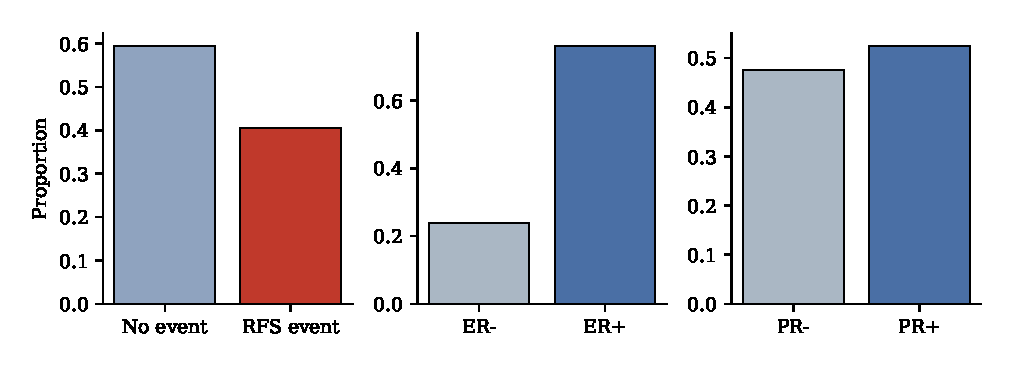
\includegraphics[width=0.62\textwidth]{figures/fig2_cohort}
\end{figure}

\begin{figure}[h]
\centering
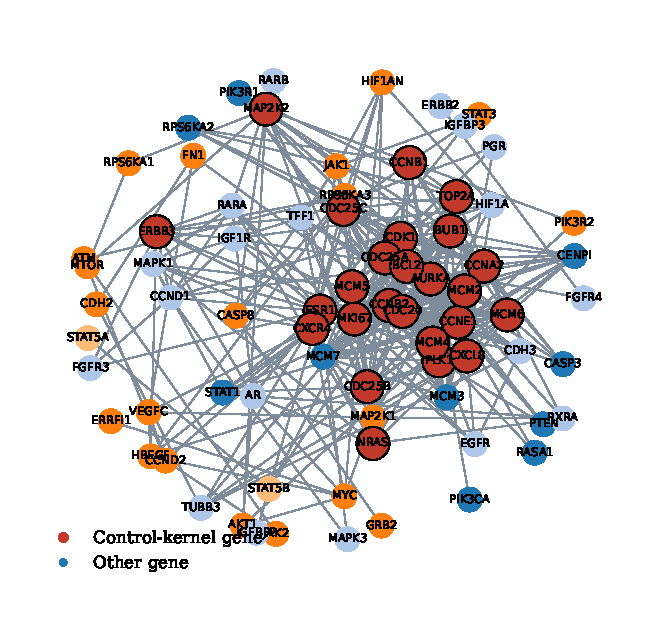
\includegraphics[width=0.85\textwidth]{figures/fig3_network}
\end{figure}

\begin{figure}[h]
\centering
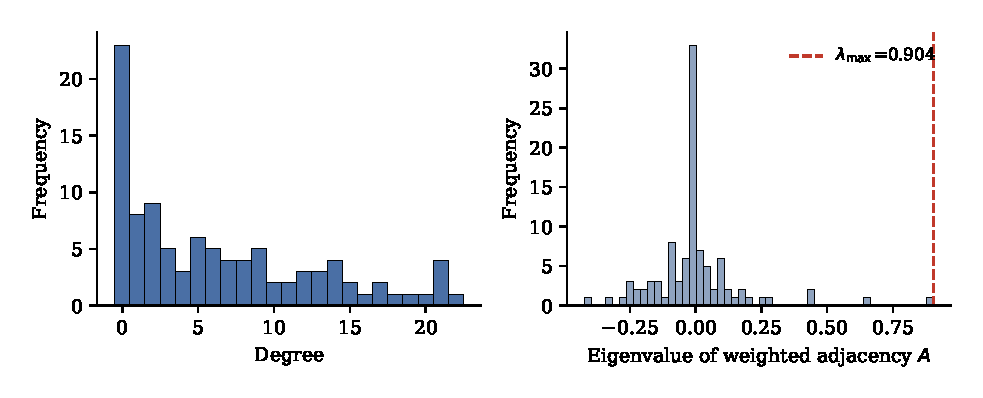
\includegraphics[width=0.62\textwidth]{figures/fig4_topology_spectrum}
\end{figure}

\begin{figure}[h]
\centering
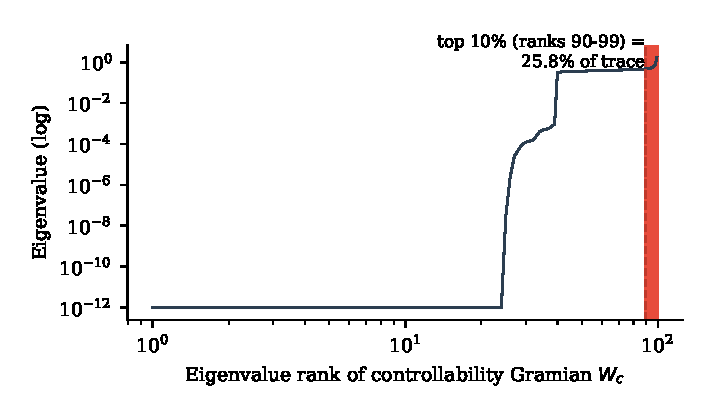
\includegraphics[width=0.62\textwidth]{figures/fig5_energy_spectrum}
\end{figure}

\begin{figure}[h]
\centering
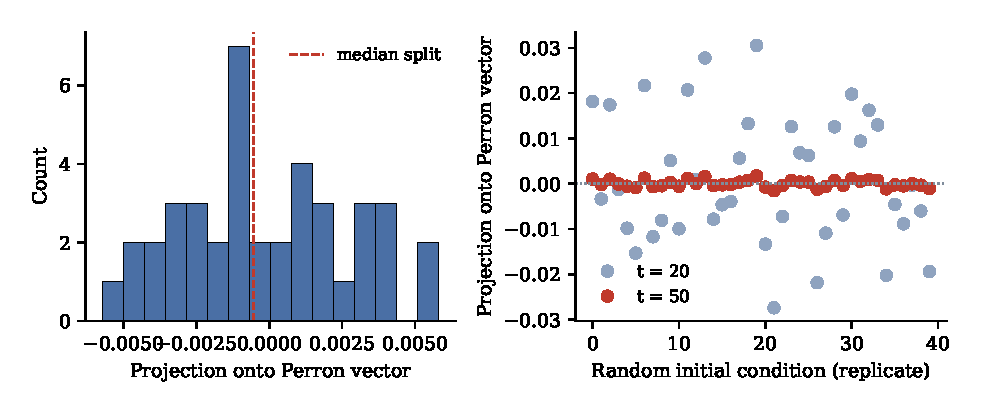
\includegraphics[width=0.85\textwidth]{figures/fig6_attractors}
\end{figure}

\begin{figure}[h]
\centering
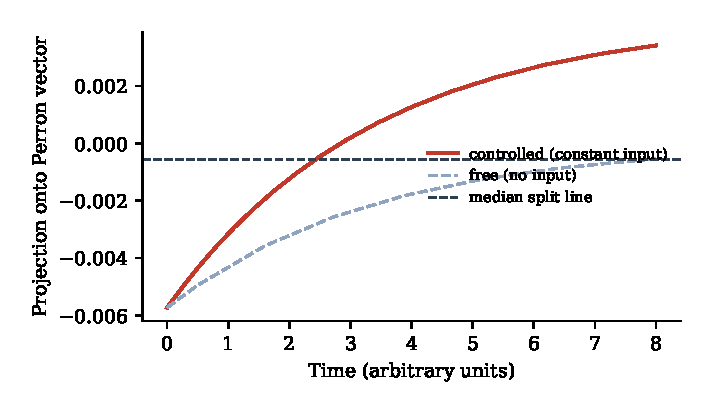
\includegraphics[width=0.62\textwidth]{figures/fig7_steering}
\end{figure}

\begin{figure}[h]
\centering
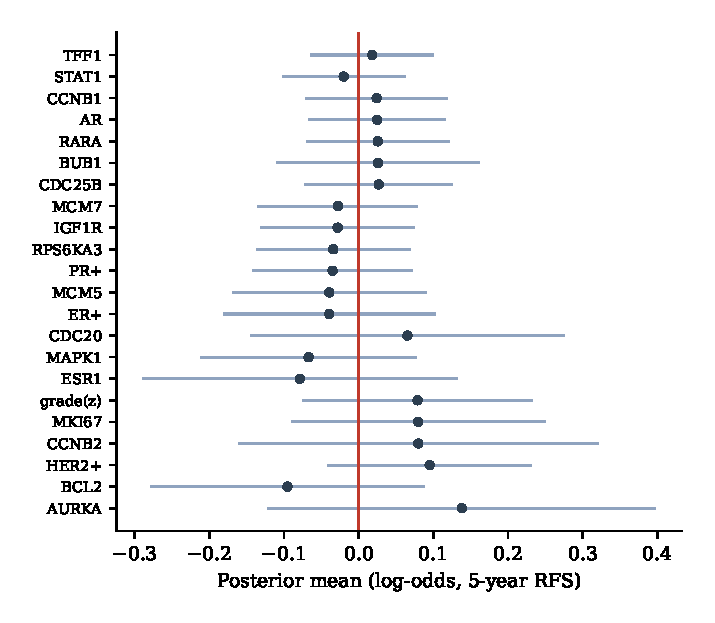
\includegraphics[width=0.62\textwidth]{figures/fig11_bayes}
\end{figure}

\begin{figure}[h]
\centering
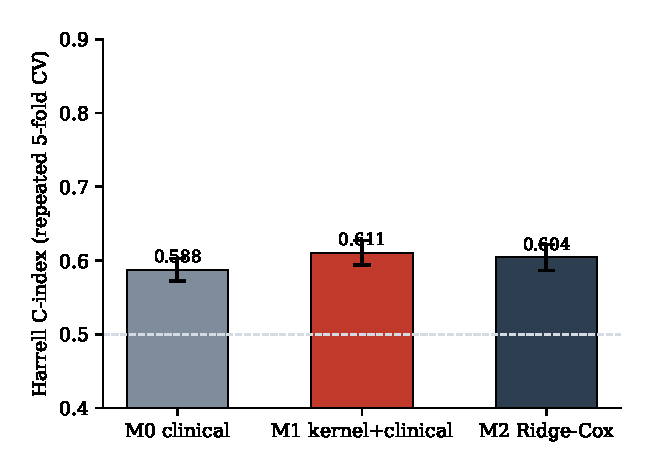
\includegraphics[width=0.62\textwidth]{figures/fig8_cindex}
\end{figure}

\begin{figure}[h]
\centering
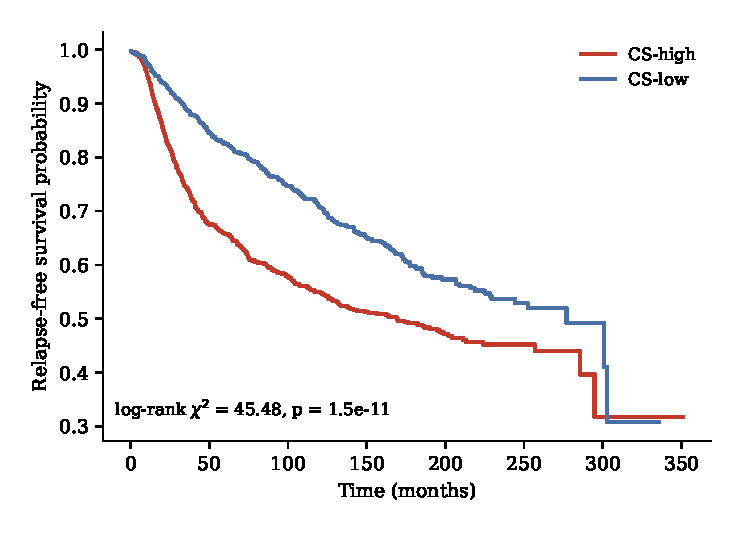
\includegraphics[width=0.62\textwidth]{figures/fig9_km}
\end{figure}

\begin{figure}[h]
\centering
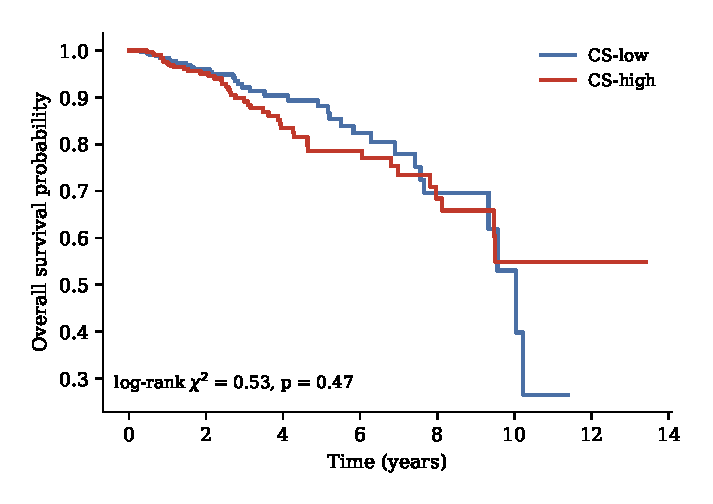
\includegraphics[width=0.62\textwidth]{figures/fig12_tcga_km}
\end{figure}

\begin{figure}[h]
\centering
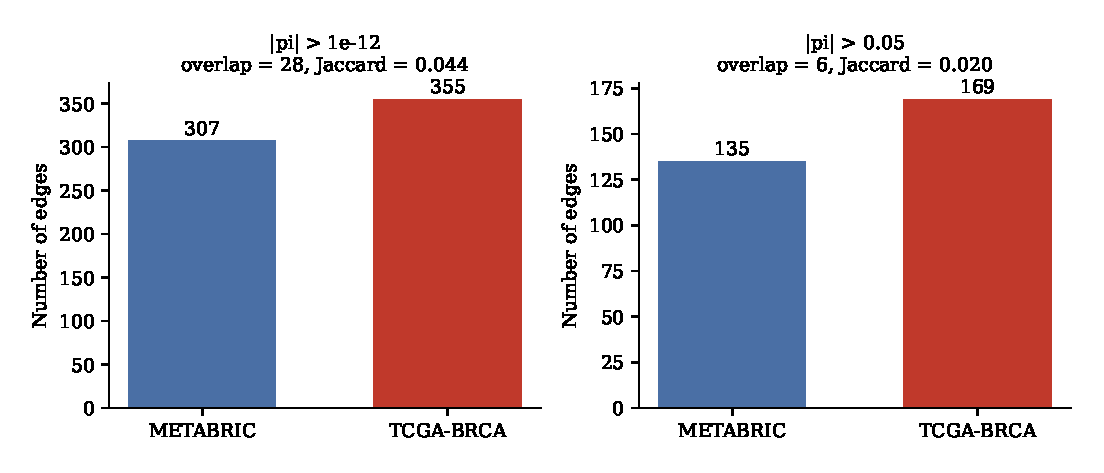
\includegraphics[width=0.62\textwidth]{figures/fig13_network_overlap}
\end{figure}

\begin{figure}[h]
\centering
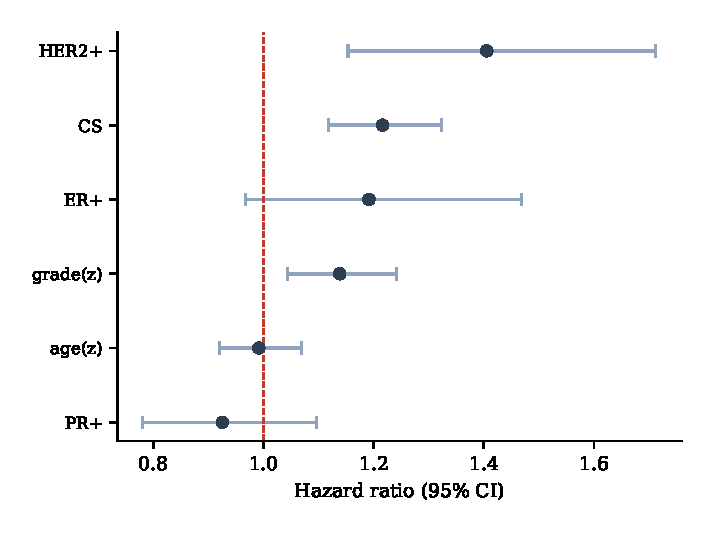
\includegraphics[width=0.62\textwidth]{figures/fig10_forest}
\end{figure}

\end{document}
